\documentclass[9pt,twocolumn,twoside]{gsajnl}
% Use the documentclass option 'lineno' to view line numbers

%\usepackage[colorinlistoftodos]{todonotes} % comments in margins
%\setlength{\marginparwidth}{1.25cm}
\definecolor{flame}{rgb}{0.89, 0.35, 0.13}
\newcommand{\josh}[1]{\textcolor{flame}{\emph{\scriptsize {#1}}}}

\articletype{gos} % article type
% {inv} Investigation
% {gs} Genomic Selection
% {goi} Genetics of Immunity
% {gos} Genetics of Sex
% {mp} Multiparental Populations

\title{Reduced Nucleotide Diversity on a Plant Y Chromosome Following Recent Recombination Suppression}

\author[$\ast$,$\dagger$,1]{Josh Hough}
\author[$\dagger$]{Felix Baudry}
\author[$\dagger$]{Wei Wang}
\author[$\dagger$]{Spencer C.H. Barrett}
\author[$\dagger$]{Stephen I. Wright}

\affil[$\ast$]{Department of Plant Sciences, University of California, Davis}
\affil[$\dagger$]{Department of Ecology and Evolutionary Biology, University of Toronto}

%\affil[$\dagger$]{Author two affiliation}
%\affil[$\ddagger$]{Author three affiliation}
%\affil[$\S$]{Author four affiliation}
%\affil[$\ast\ast$]{Author five affiliation}

\keywords{Sex Chromosome Evolution; Nucleotide Diversity; Recombination; Deleterious Mutations}

\runningtitle{Plant sex chromosome evolution} % For use in the footer

\correspondingauthor{Josh Hough}

\begin{abstract}
X and Y chromosomes differ in effective population size ($N_{e}$), rates of recombination, and exposure to natural selection, all of which can significantly affect levels of genetic variability within the genome. On Y chromosomes with suppressed recombination, both positive and negative selection can reduce the frequencies of genetically linked neutral variants, resulting in a reduction in $N_{e}$ and the level of neutral polymorphism on Y compared to X chromosomes or autosomes. However, non-selective factors including biased sex ratios and high variance in male fitness can also reduce Y-linked $N_{e}$, making it difficult infer the causes of low Y-chromosome diversity. Here, we investigate the factors affecting X- and Y-linked polymorphism during the early stages of plant sex chromosome evolution in \textit{Rumex hastatulus} (Polygonaceae). Strikingly, our analysis revealed that nucleotide diversity on the Y is approximately 12.5 fold lower than predicted from models of neutral evolution. We demonstrate that the magnitude of this reduction is unlikely to be explained by the observed occurrence of female biased sex ratios in this species, or by reduced male $N_{e}$ caused by high variance in male fitness. Rather, using forward simulations, we show that the diversity reduction on the Y is consistent with the predicted effects of background selection arising from suppressed recombination. Given the recent origin of \textit{R. hastatulus} sex chromosomes, our results indicate that the low level of sequence diversity commonly observed on ancient Y chromosomes might evolve soon after sex chromosomes originate, with background selection playing an important role during the early stages of their evolution.

%this is 254 words and cannot be any longer than 250. Make edits accordingly.

%Add citations using the \verb|\citep{}| command, for example \citep{neher2013genealogies} or for multiple citations, \citep{neher2013genealogies, rodelsperger2014characterization}

\end{abstract}

\setboolean{displaycopyright}{true}

\begin{document}

\maketitle
\thispagestyle{firststyle}
\marginmark
\firstpagefootnote
\correspondingauthoraffiliation{jhough@ucdavis.edu}
\vspace{-11pt}%

\section*{Introduction}

\lettrine[lines=2]{\color{color2}M}{}orphologically distinct sex chromosomes have evolved multiple times independently in both plant and animal kingdoms \citep{westergaard1958,ohno1967,bull1983,charlesworth1991}. Despite numerous biological differences between the kingdoms, X and Y chromosomes in both lineages have undergone similar genetic changes, suggesting that general evolutionary mechanisms might drive sex chromosome divergence \citep{charlesworth1978,charlesworth1996CB,charlesworth2000degeneration}. Investigating the shared features of plant and animal sex chromosomes, including the loss of recombination \citep{bergero2009}, the degeneration of Y chromosomes \citep{hough2014,bergero2015}, and the evolution of dosage compensation \citep{muyle2012,papadopulos2015}, thus provides an informative context for investigating the evolutionary forces driving sex chromosome evolution.

One fundamental difference between sex chromosomes and autosomes is their respective copy number in a population; whereas autosomes in diploid species are present in two copies in each sex, the X chromosome is present in two copies in females and only one copy in males. As a consequence, the effective population size ($N_{e}$) of the X chromosome is predicted to be 3/4 that of autosomes, whereas the $N_{e}$ of the male-limited Y chromosome is expected to equal 1/4 that of autosomes (assuming an equal number of reproducing females and males). Such differences in $N_{e}$ are predicted to directly affect relative levels of neutral polymorphism maintained on these chromosomes, which is proportional to the product of $N_{e}$ and the neutral mutation rate, $\mu$ \citep{Kimura1984}. This variation in neutral polymorphism is in turn expected to have important consequences on patterns of DNA sequence evolution, including the effectiveness of both positive and negative selection \citep{charlesworth1987}.

Several demographic factors are expected to modulate or accentuate differences in polymorphism levels maintained on sex chromosomes \citep{ellegren2009}. These include population subdivision and sex-biased dispersal, deviations from a 1:1 breeding sex ratio, and high variance in reproductive success \citep{caballero1995,charlesworth2001,laporte2002,pool2007}. For example, studies comparing levels of variability on the X chromosome and autosomes in humans have found evidence that sex-biased dispersal has reduced levels of X-to-autosome diversity below the neutrally expected level of 0.75 \citep{keinan2009}, though there is considerable variation in current estimates of the X/A ratio in humans, and other demographic processes have also been suggested \citep{hammer2010,bustamante2009}. Theoretical work also indicates that population bottlenecks can lead to disproportionate decreases in sex-linked compared to autosomal variation \citep{pool2007}, a prediction that has been supported in a diverse array of taxa, including chimpanzees and orangutans \citep{kaessmann2001,fischer2006}, the house mouse \textit{Mus musculus} \citep{baines2007}, Drosophila \citep{andolfatto2001}, and humans \citep{keinan2009}.

In addition to demographic factors, evolutionary theory predicts that genetic variability on sex chromosomes should also be affected by the evolution of suppressed X-Y recombination, which lowers the coalescent $N_{e}$ for Y-linked genes and increases their vulnerability to the effects of selective sweeps \citep{smith1974hitch,aquadro1994} and background selection \citep{charlesworth1996background,charlesworth1994effect}. These processes can be viewed as examples of the Hill–Robertson (HR) effect, in which the effective population size for a given chromosomal region depends strongly on the rate of recombination, such that selection at a focal site is not independent of selection at nearby sites \citep{hill1966HReffect}. Moreover, both the background selection and selective sweep models predict a reduction in $N_{e}$ and, as a result, reduced levels of neutral polymorphism, selection efficacy, and rate of adaptation \citep{comeron2008}. Although the HR effect can occur throughout the genome \citep{mcvean2000}, large genomic regions in which recombination is suppressed, such as the Y chromosome, are expected to experience the most severe reductions in neutral diversity due to chromosome-wide linkage \citep{charlesworth1996CB,charlesworth2000degeneration,bachtrog2013NRG}. Consistent with this, studies examining Y chromosome variability in mammals \citep{hellborg2004,Wilsonsayres2014} and Drosophila \citep{mcallister1999,bachtrog2000} have found that Y-linked diversity is considerably lower than predicted under models of neutral evolution, suggesting that the HR effect plays a key role determining patterns of nucleotide diversity during sex chromosome evolution across a broad range of animal taxa.

Despite widespread interest in determining the effects of recombination on patterns of genetic diversity and the forces contributing to sex chromosome divergence \citep{ellegren2011,otto2011PAR,bachtrog2013NRG}, we still know little about the influence of the HR effect on patterns nucleotide polymorphism in young sex chromosome systems, where \textit{de novo} recombination suppression has evolved relatively recently \citep{charlesworth2016plant}. The timescales over which selection affects neutral polymorphism on sex chromosomes is therefore not well understood. Recent studies of young sex chromosome system in plants have revealed that several canonical features of X and Y chromosome evolution are shared between plants and animals, including the genetic deterioration of the Y chromosome \citep{bergero2015,hough2014}, the occurrence of ‘evolutionary strata’ \citep{bergero2009}, and the evolution of dosage compensation \citep{muyle2012,papadopulos2015}. Nonetheless, except for a small number of genes in \textit{Silene latifolia} \citep{filatov2001diversity,qiu2010nucleotide}, the associated changes in genetic diversity that are predicted from evolutionary models of X- and Y-chromosome evolution have not been widely studied in young plant sex chromosomes. Given that both background selection and selective sweeps are predicted to have the strongest effects during the earliest stages of Y-chromosome evolution, before Y-chromosomes have lost a large proportion of their genes \citep{bachtrog2008temporal}, studying recently evolved plant sex chromosomes provides an important test of the temporal dynamics of the HR effect.

To investigate the factors affecting nucleotide diversity in the early stages of sex chromosome evolution, we analyzed single nucleotide polymorphisms (SNPs) on sex chromosomes and autosomes in the plant \textit{R. hastatulus }(Polygonaceae). This species is a dioecious annual with highly heteromorphic X and Y chromosomes that are estimated to have evolved  approximately 15 MYA \citep{quesada2011,grabowska2015,navajas2005}, making sex chromosomes in this species over 100 million years younger than those in mammals \citep{lahn1999,ross2005dna}. \textit{Rumex hastatulus} has received particular attention because of the unique occurrence of an intraspecific polymorphism for sex chromosome system, in which both XY and $XY_{1}XY_{2}$ males occur in geographically distinct chromosomal races \citep{smith1963mechanism}. The $XY_{1}XY_{2}$ sex chromosome system (the North Carolina race) is thought to have originated through an X-autosome fusion, with the XY system (the Texas race) maintaining the ancestral chromosome complement \citep{smith1964evolving}. Despite the recent origin of the sex chromosome systems in this species, there is evidence that both the ancestral and neo-Y chromosomes have undergone significant genetic degeneration, though less degeneration was inferred for younger sex-linked genes unique to the North Carolina race \citep{hough2014}.

Of particular relevance to the present study is that \textit{R. hastatulus} populations throughout their geographical range (southern USA) consistently exhibit female-biased sex ratios, with a mean sex ratio of $N_{m}/N_{f}=0.6$ \citep{pickup2013influence}. This is important because female-biased sex ratios are predicted to affect levels of sex chromosome diversity \citep{ellegren2009}, though few studies have attempted to empirically distinguish between the effects of biased sex ratios and selective interference. Here, focusing on the $Y_{1}$ chromosome that is shared between the chromosomal races of \textit{R. hastatulus}, we tested whether levels of nucleotide diversity on X, Y, and autosomal chromosomes were jointly consistent with predictions from models of sex ratio bias and variance in reproductive success. In addition, we use population genetic parameters estimated from our data to conduct forward-time simulations of both purifying and positive selection to determine the relative support for models of background selection and selective sweeps in explaining the levels of diversity we observed.

\section*{Materials and Methods}
\subsection*{Population Samples and Sex-Linked Genes}
We analyzed sex-linked and autosomal genes identified from Illumina RNA sequence data from 24 individuals (12 males and 12 females, with 1 male and 1 female from each of 12 populations, 6 populations of each sex chromosome race). Samples of both sex chromosomal races were collected in 2010 from throughout the native range of \textit{R. hastatulus} (locations in Table S1), and plants were grown in the glasshouse from seeds collected from open-pollinated females. We extracted RNA from leaf tissue using Spectrum Plant Total RNA kits (Sigma-Aldrich). The isolation of mRNA and cDNA synthesis was conducted according to standard Illumina RNAseq procedures, with sequencing conducted on two Illumina HiSeq lanes with 150-bp end reads at the Genome Quebec Innovation Center. Reads from these 24 samples were mapped to the \textit{R. hastatulus} reference transcriptome \citep{hough2014}, and raw sequences are available from the Gen-Bank Short Read Archive under accession no. SRP041588. Reads were mapped using the Burrows–Wheeler Aligner (release 0.6.2-r126 \citep{li2010fast}), followed by Stampy (release 1.0.20; \citep{lunter2011stampy}). We used Picard tools (release 1.78, http://picard.sourceforge.net) to modify mapping output into the format required for the Genome Analysis Toolkit (GATK version 2.1-11; \citep{mckenna2010genome}) variant calling software, and subsequently removed genes with low coverage (<10x) and Phred Quality Scores (<20). The population samples analyzed here were previously reported in Hough et al. (2014), where they were used to validate the ascertainment of sex-linked contigs identified through segregation analysis. From the list of sex-linked genes identified in Hough et al. (2014) that were shared between the Texas (XY) and North Carolina (XY1Y2) sex chromosome races, we identified a total of 460 sex-linked genes for analysis.

\subsection*{Autosomal Genes}
In evaluating evidence for nucleotide diversity differences between X and Y chromosomes, it is important to distinguish between reduced Y-linked diversity, and the possibility that X-linked diversity is elevated above the level predicted from a neutral model. To do this, we normalized sex-linked diversity estimates by autosomal diversity, and compared empirical X/A and Y/A nucleotide diversity ratios to those predicted from a neutral model (described below). Because the criteria for identifying autosomal loci in Hough et al. (2014) were based on the occurrence of four segregating SNPs per locus, and this set is therefore probably higher in diversity than the average autosome, here we incorporated a broader set of all non-sex linked (punitively autosomal) genes from our transcriptome data. We filtered this set of non-sex linked genes to remove those that may have been sex-linked but were not identified as such by the ascertainment criteria in Hough et al. (2014). In particular, we removed: (i) any genes in which there was evidence for at least one SNP with a sex-linked segregation pattern, (ii) any genes with SNPs showing fixed heterozygosity in males and fixed homozygosity in females, (iii) any genes with less than 10X coverage or greater than 100X coverage from independently obtained genomic coverage data (to filter out duplicate genes or those with highly repetitive sequences), and (iv) any genes containing SNPs with large (>0.4) allele frequency differences between males and females. Finally, we removed genes with fewer than 100 synonymous sites following filtering to avoid biasing results toward genes that may have been particularly short due to assembly problems. This filtering resulted in a set of 12,356 and 11,350 autosomal genes in the Texas and North Carolina races, respectively.

\subsection*{Phasing X and Y alleles}
To estimate polymorphism for the X and Y sequences separately, it is necessary to infer the phase of SNPs in sex-linked transcripts in males. In previous work, phasing alleles on \textit{R. hastatulus} sex chromosomes was achieved using segregation analysis from a genetic cross. Here, to phase SNPs from population samples where such segregation data was unavailable, we used HAPCUT \citep{bansal2008hapcut}, a maximum-cut based algorithm that reconstructs haplotypes using sequenced fragments (Illumina read data) from the two homologous chromosomes in a diploid individual to output a list of phased haplotype blocks containing the SNP variants on each chromosome. Because the resulting haplotype blocks produced by HAPCUT contained SNPs that were phased relative to each other, but not designated to either the X or Y chromosome, we assigned individual variants to X or Y by independently identifying fixed X-Y differences with each haplotype block (i.e., sites in which all females were homozygous, and all males were heterozygous). Identifying such fixed differences within phased haplotype blocks enabled us to then infer the correct phase (X or Y) of the polymorphisms from HAPCUT’s output. This was done by matching the phase of fixed X-Y differences with their neighboring polymorphic sites - i.e., when a fixed X-Y difference occurred in the same phased haplotype block as a polymorphic site, the polymorphic variants in that block were assigned to either X or Y based on the known phase of the fixed difference with which they were matched. SNPs that were identified outside of phased blocks, or in blocks without fixed X-Y differences, were recorded as missing data. Finally, we filtered SNPs for coverage > 60, QUAL score > 60, and those within a distance of 10bp or less from indels. This procedure was conducted using a combination of Perl and Bash and this resulted in fasta-formatted alignments of X and Y sequences for 372 sex-linked genes from the 24 individuals in our study.

We further validated the results of HAPCUT’s allele phasing by comparing the accuracy of this method with the phasing-by-segregation method that was conducted using data from a genetic cross in Hough et al. (2014). To do this, we first phased the sequence data from parents and their progeny using HAPCUT’s algorithm (using the same parameters as for the population data). In particular, we looked for cases where SNPs were inferred on the Y chromosome by HAPCUT, but where the ‘true’ level polymorphism was zero, since Y-linked  sequences from a single family should all be identical, as we had confirmed through phasing by segregation. We identified 7 percent of sex-linked genes that had phasing errors of this kind, or that we determined to have genotyping errors resulting in a false SNP calls on the Y chromosome, leading to a SNP error rate estimate of 1.7 x 10-4. This rate is very low relative to the population-based estimates of polymorphism on the X and autosomes (Table 1), and therefore should have minimal effects on our estimation of X/A polymorphism. However, because this rate is high relative to the expected level of true polymorphism on the Y-chromosome, we further filtered genes in which we found evidence for false-positive Y-polymorphisms arising from: (i) phasing errors caused by gene duplicates (more than two haplotypes), (ii) polymorphisms around indels, and (iii) genotyping errors caused by low Y-expression. This filtering was done by manually inspecting sequences in IGV \citep{robinson2011integrative} and identifying each individual putative polymorphism on the Y chromosome.

\subsection*{Estimating neutral polymorphism on sex chromosomes and autosomes}
For each locus in our analysis, we calculated Watterson’s (1975) estimator of the population parameter $\theta=4N_{e}\mu$, where $N_{e}$ is the effective population size, and $\mu$ is the mutation rate \citep{watterson1975}, using a modified version of the Perl program Polymorphurama \citep{bachtrog2006}. To compare sex-linked and autosomal loci, we calculated the average value of $\theta$, weighted by the number of synonymous sites in each gene (Figure 2; Table 1). ). We obtained 95 percent confidence intervals for our estimates of the X/A and Y/A diversity ratios by bootstrapping by gene using the BCa method \citep{efron1994} implemented in the Boot package in R \citep{canty2012boot}, and calculating X/A and Y/A diversity on each iteration for 20000 replicates each. Bootstrapping was conducted on the final filtered set of 173 sex-linked, and 12355 autosomal genes from the Texas race, and separately for the 176 sex-linked and 11349 autosomal genes from the North Carolina race. Note that the lack of recombination on the Y chromosome implies that assumptions of independence are likely violated, since Y-linked loci are expected to be non-independent, and therefore the true uncertainty in our Y/A diversity estimate obtained by this method is likely an underestimate. To address this issue, we used a maximum likelihood approach implemented in the software \citep{wright2004hka} to obtain independent estimates of the Y/A ratio. Here, [explain more]. Finally, we also tested whether estimates of diversity on the X chromosome calculated from females were consistent with estimates from phased X sequences from males. As no significant difference was observed, we report only results from females.

\subsection*{Neutral predictions and the effect of sex ratio bias on diversity}
Wright's (1931) formula $N_{e}=4N_{f}N_{m}/(N_{f} + N_{m})$ gives the effective population size of a randomly mating population with separate sexes and a Poisson distribution of offspring number. For a female effective population size $N_{f}$, and a male effective population size $N_{m}$, the predicted effective population size for X-linked genes relative to autosomes is given by $N_{e_{X}}/N_{e_{A}} = 9(N_{f}+N_{m})/8(2N_{f}+N_{m})$ (Wright 1931). In a neutral model with equal sex ratios, $N_{e_{X}}/N_{e_{A}} = 0.75$. For populations with female-biased sex ratios, however, $N_{m}$ becomes small relative to $N_{f}$ and this ratio can become larger than 1, approaching 1.125 at the limit \citep{caballero1995}. For the Y chromosome, the effective population size is given by 1/4 the total $N_{e}$ or 1/2 the $N_{e}$ of males, $N_{m}$/2. Under neutrality, the level of nucleotide polymorphism maintained in a population is proportional to the product of the mutation rate and the effective population size: $\theta=4N_{e}\mu$ \citep{watterson1975,kimura1984}. Assuming equal neutral mutation rates for all genes and an equal number of reproducing males and females, Y-linked genes should therefore have 1/3 the polymorphism of X-linked genes, and 1/4 that of autosomal genes. Figure 1 shows the predicted relative effective population size ratios for autosomal, X-linked, and Y-linked genes (left) and the corresponding X/A and Y/A ratios of diversity (right) for a sex ratio bias ranging from $N_{f}/(N_{f}+N_{m})=0$ to $N_{f}/(N_{f}+N_{m})=1$.

\begin{figure}[htbp]
\centering
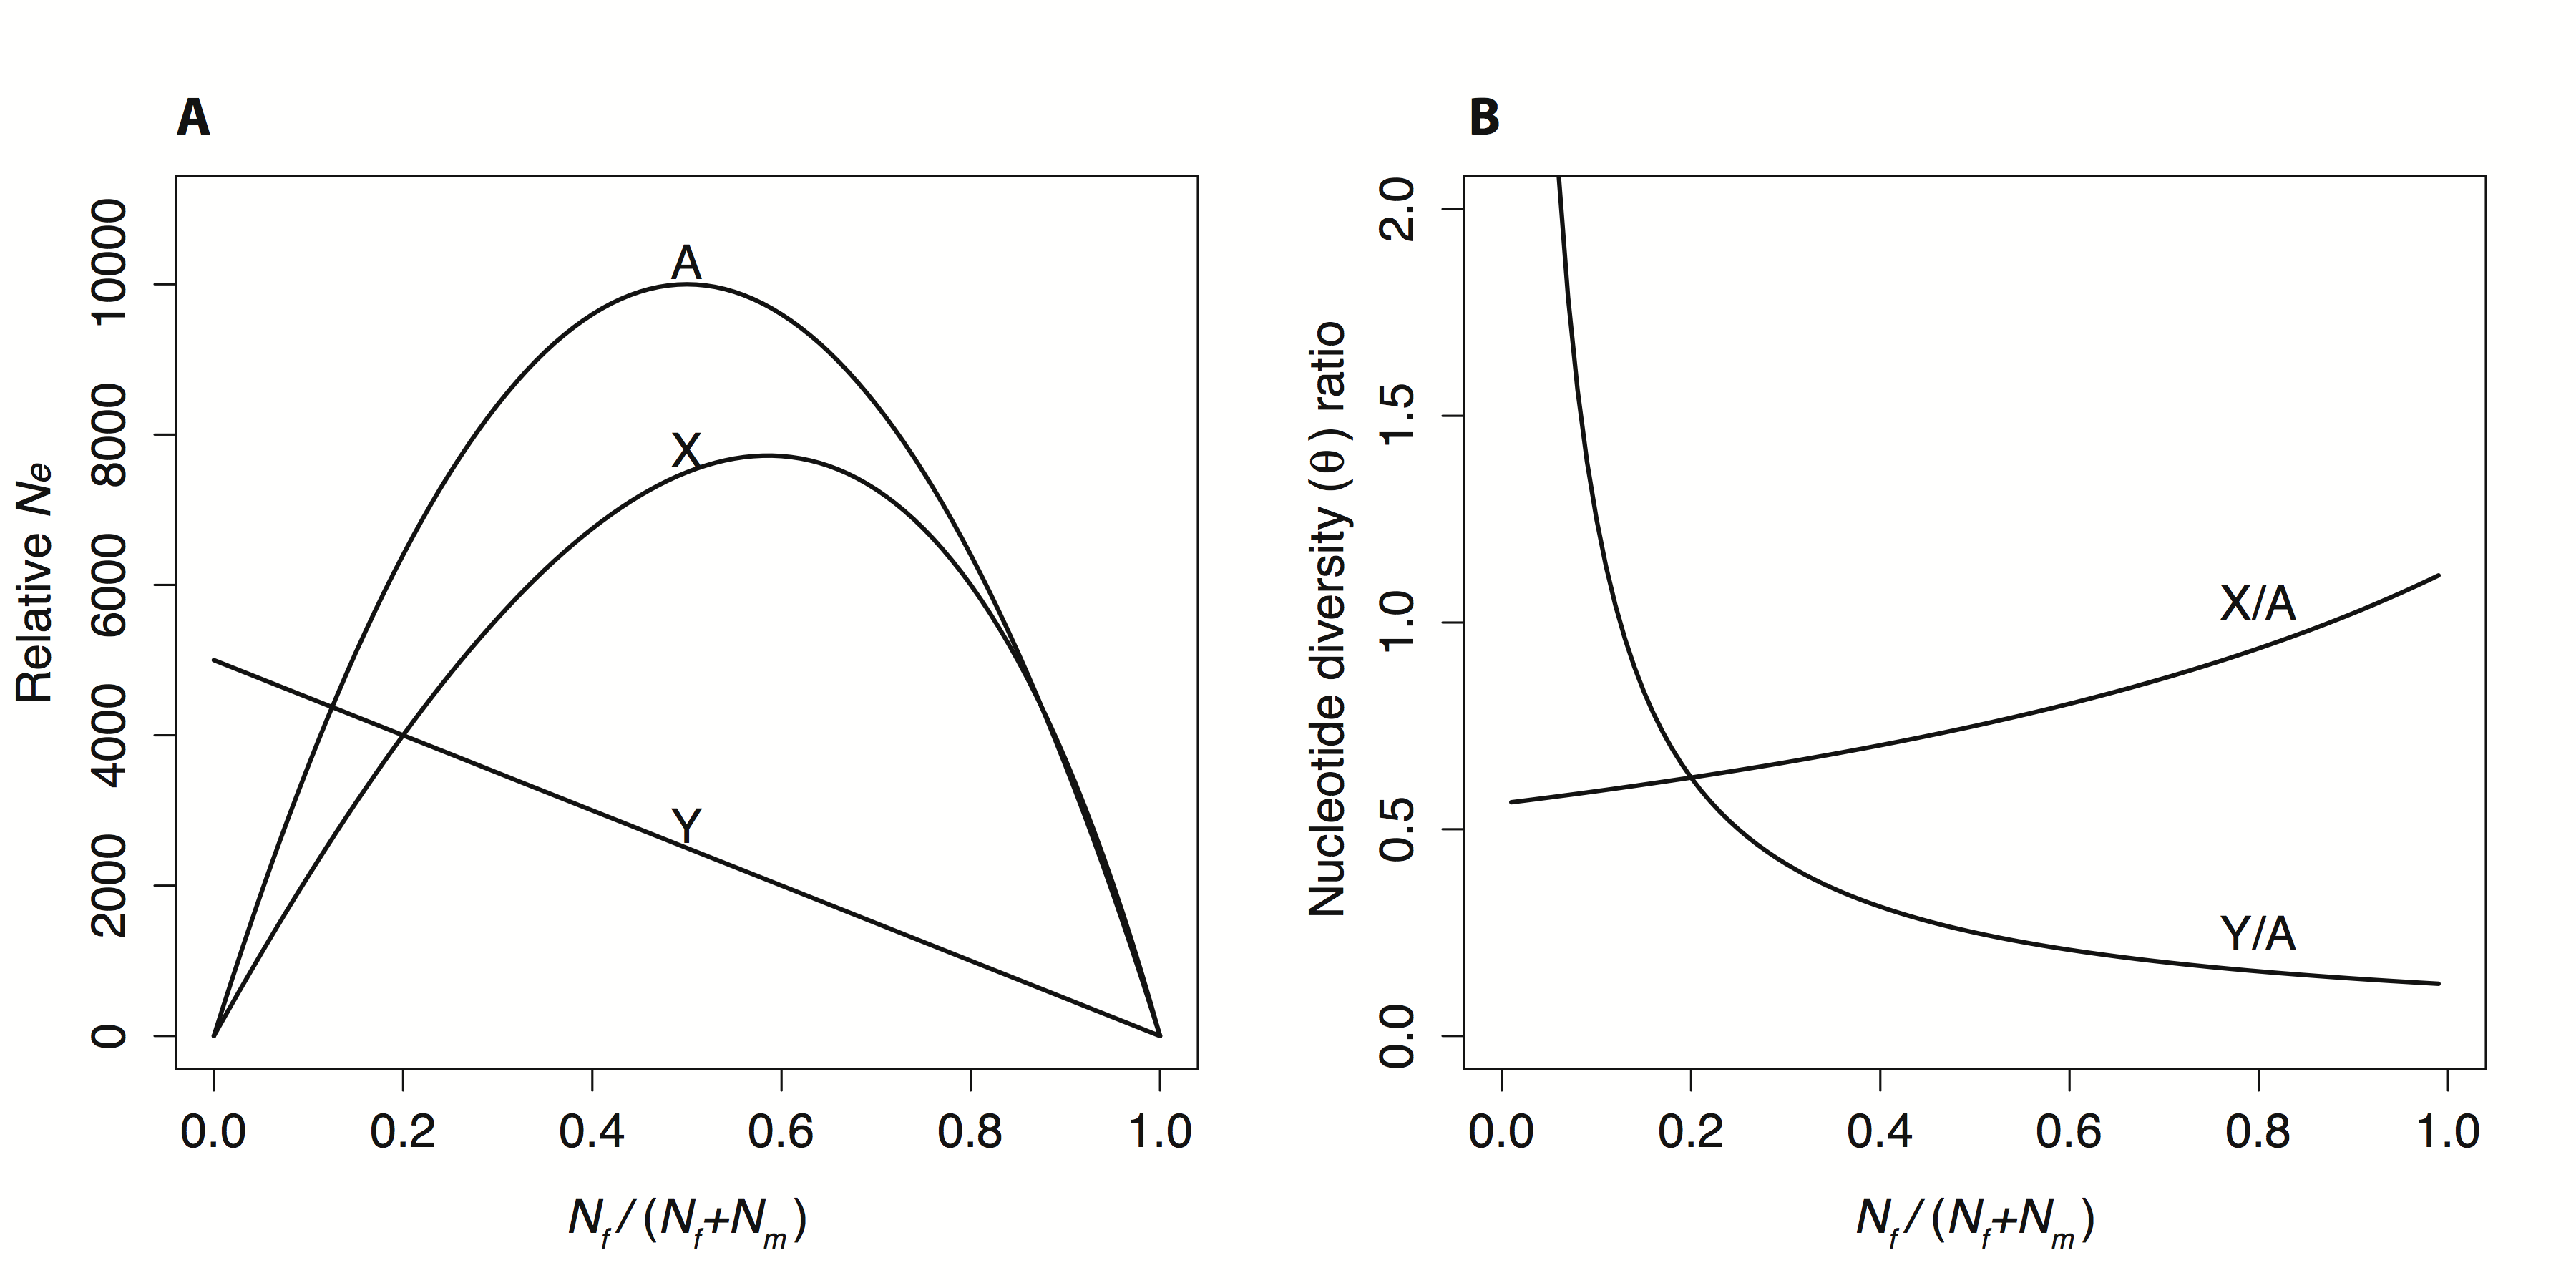
\includegraphics[width=\linewidth]{Figure1.png}
\caption{\textbf{A:} The relation between relative effective population size and sex ratio bias for genes on autosomes (A), X chromosomes (X), and Y chromosomes (Y). The sex ratio is shown as the proportion of females, $N_{f}/(N_{f}+N_{m})=0$, ranging from 0 to 1, where $N_{m}$ and $N_{f}$ are the effective number of breeding males and females, respectively. Calculations assume a constant population size, non-overlapping generations, and a Poisson distribution of offspring number \citep{wright1931evolution,charlesworth2009effective}. The $N_{e}$ for each chromosome type is calculated relative to the predicted $N_{e}$ for genes on autosomes with an equal sex ratio.\textbf{B:} The corresponding expected relation between sex ratio bias and the sex-chromosome-to-autosome diversity ratio, assuming $\theta=4N_{e}\mu$ and equal neutral mutation rates for all genes.
}%
\label{fig:spectrum}
\end{figure}

\subsection*{Simulations of Background Selection and Selective Sweeps}
To investigate whether our observed level of Y-chromosome diversity could be explained by background selection, we conducted forward time simulations..a 


\josh{
\textit{to do}
\begin{itemize}
\item \textit{describe parameters used and justify}
\item \textit{do both purifying and positive selection sims}
\end{itemize}
}

We modeled both purifying and positive selection using the forward simulation software SFS_CODE \citep{hernandez2008flexible}. To make the simulation output more comparable to our data, we used estimates of $\theta$ from our polymorphism data ... A with our empirical sampling, the simulations sampled 8 chromosomes per simulation. 

%using the software packages fwdpp and fwdpy (Thornton, 2014), and analyzed the output using libsequence (Thornton 2003) and standard Python. To match the sample size of our empirical data, we simulated sex chromosomes and autosomes from 24 individuals , and collected diversity statistics after evolving populations under background selection for 10N generations with 1000 replicates each. To consider only the effects of selection against deleterious alleles, we ignored adaptive mutations and sampled selective coefficients from a gamma distribution with shape parameter 0.1, mean selection coefficient s = -0.01, neutral mutation rate μ = 0.005, deleterious mutation rate U = 0.01 (diploid), and dominance term h = 1 . Our simulations assumed that recombination did not occur on Y-chromosomes, whereas we allowed X chromosomes and autosomes to experience free recombination uniformly throughout their length. Initial effective population sizes for simulated sex chromosomes were set such that NeX/NeA = 3/4 and NeY/NeA = 1/4, with an initial NeA of 1000. To compare the simulation output with our empirical data, we calculated the average θ over all simulations, and calculated normalized X/A and Y/A ratios of neutral diversity (Figure 2). Confidence intervals were calculated from bootstrapping 10000 replicate simulations  using the BCa method (Efron 1987) implemented in the Boot package in R (Canty and Ripley 2012; R Core Team 2011). 



\begin{equation}
S_n = \frac{X_1 + X_2 + \cdots + X_n}{n}
      = \frac{1}{n}\sum_{i}^{n} X_i
\label{eq:refname1}
\end{equation}


\section*{Results and Discussion}

\subsection*{Evolutionary relationships of sex chromosome races in \textit{R. hastatulus}}

\subsection*{Male-to-female sex ratio of $N_{e}$}

\subsection*{Background Selection and Selective Sweeps}

\section*{Conclusions}
\section*{Acknowledgments}


\bibliography{bibliography}
\end{document}
